\section{Week 8}
\textbf{\large \underline{Direct Analytic Design / Ragazzini's Method:}}
\vspace{0.25cm}

The proposed controller $G_c(z)$ is,
\begin{align*}
    G_c (z) &= \frac{1}{G_p(z)}\cdot \frac{F(z)}{1-F(z)} \\
    &= \frac{D_p(z)}{N_p(z)}\cdot \frac{N_F(z) / \cancel{D_F(z)}}{N_{1-F}(z)/\cancel{D_{F}(z)}} \\
    &= \frac{D_p(z)}{N_p(z)}\cdot \frac{N_F(z)}{N_{1-F}(z)}
\end{align*}

\textbf{Important Remarks}
\begin{enumerate}
    \item Any undesirable poles in the plant must be cancelled by terms in $N_{1-F}(z)$;
    \item Any undesirable zeros in the plant must be cancelled by terms in $N_F(z)$.
    \item $F(z)$ is the desired transfer function and it is already KNOWN.
\end{enumerate}

\textbf{\large \underline{Pole-Zero Deficiency:}}
\begin{enumerate}
    \item Definition:
    \begin{align*}
        d_f = \mathcal{D}\{F(z)\} &\eqdef  \text{Order}\{D_{F}(z)\} - \text{Order}\{N_{F}(z)\} \\
        \mathcal{D}\{G_p(z)\} &= d_p \\
        \mathcal{D}\{G_{c}(z)\} &= d_f - d_p - 0 
    \end{align*}
    \item \textbf{Causality Constraint:} $\mathcal{D}\{F(z)\} \geq \mathcal{D}\{G_p(z)\}$. In other words, the controller must be either proper ($d_f = d_p$) or strictly proper ($d_f -d_p >0$) for it to be implementable.
\end{enumerate}

\textbf{\large \underline{Steady state accuracy:}}
\vspace{0.25cm}

For $\frac{Y(z)}{U(z)}=F(z)$, the accuracy is measured by:
\begin{table}[H]
\centering
\renewcommand{\arraystretch}{2}
\begin{adjustbox}{max width=\textwidth}
\begin{tabular}{|c|c|c|}
\hline
\textbf{Type of Input} & \textbf{Accuracy is measured by}  & \textbf{Condition}  \\\hline
Unit Step,             & \multirow{2}{*}{steady state error $E_{ss}$} & \multirow{2}{*}{$E_{ss} = 0$ if $F(1) = 1$}                \\ 
$U(z) = \frac{z}{z-1}$   &                                              &                                                            \\ \hline
Unit Ramp,             & velocity error $K_v$                         & $\frac{1}{T\, K_v} = -\left.\frac{dF(z)}{dz}\right|_{z=1}$ \\ \cline{2-3}
$U(z) = \frac{Tz}{(z-1)^2}$ &
  steady state error $E_{ss}$ &
  \begin{tabular}[c]{@{}c@{}}$E_{ss}=0$ if $K_v \to \infty$,\\ i.e. $\left.\frac{dF(z)}{dz}\right|_{z=1}=0$\end{tabular} \\ \hline
\end{tabular}
\end{adjustbox}
\end{table}

\textbf{Remarks on Velocity Error $K_v$:}

\begin{itemize}
    \item Useful definition when doing $G_c$ design: 
    \begin{equation*}
        K_v\eqdef \lim_{s\to 0} s G_c(s) G_p(s)
    \end{equation*}
    \item Velocity error is usually given as a percentage. \textbf{N.B.} that a 10\% velocity error means that $\frac{1}{K_v}=0.1$, so $K_v = 10$;
    \item If want zero steady state error with unit ramp input, set $K_v \to \infty$ and solve $\left.\frac{dF(z)}{dz}\right|_{z=1} = 0$
\end{itemize}

\begin{figure}[H]
    \centering
    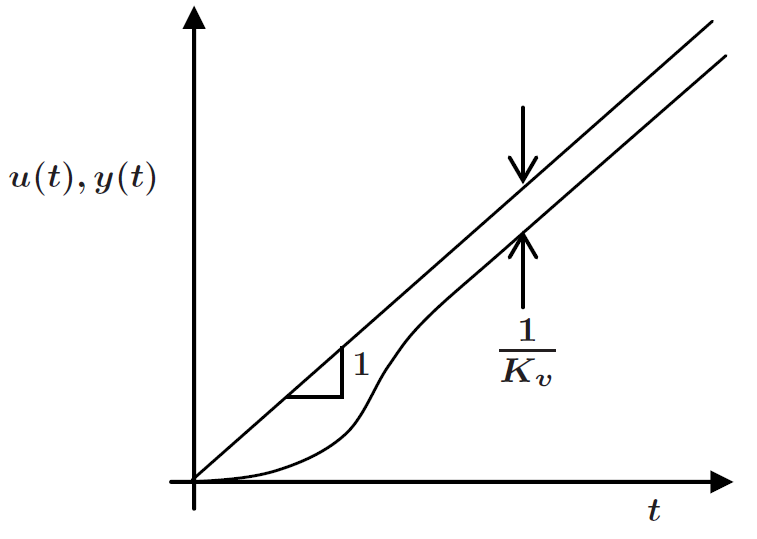
\includegraphics[width=0.75\linewidth]{images/K_v_constant.png}
    \captionsetup{justification=centering}
    \caption{Velocity error $K_v$.}
\end{figure}